\section{The advection equation}

In want to solve the following advection equation
\begin{equation}
  v_t + v v_x = 0,
  \label{eq_advection}
\end{equation}
where $v$ is velocity, $t$ is time, $x$ position, and $v_t$ is a short notation for the derivative $\frac{\partial v}{\partial t}$. We have the following initial condition
\begin{equation}
  v(x, 0) = \cos x,
  \label{eq_advection_intial_condition}
\end{equation}
and we want to solve the equation for values of $x$ and $t$ from the intervals
\begin{equation}
  -\pi < x < \pi, \quad \quad 0 \leq t \leq 1.4.
  \label{eq_x_t_ranges}
\end{equation}


\section{Using analytical solution}

Here we use analytical solution of \autoref{eq_advection}:
\begin{equation}
  v = \cos (x - v t ).
  \label{eq_analytical_solution}
\end{equation}
Our goal is to write a Fortran program that solves \autoref{eq_analytical_solution} for various values of $x$ and $t$ parameters from the intervals given by Inequalities \ref{eq_x_t_ranges}.

\subsection{Using Newton-Raphson method}

In order to solve \autoref{eq_analytical_solution} numerically, we use Newton-Raphson method:
\begin{equation}
  v_{n+1} = v_n - f(v_n, x, t) / f'(v_n, x, t),
  \label{eq_recurrence}
\end{equation}
where $n=1, 2, \dots, N_{max}$ is the iteration number with $N_{max}$ being the maximum number of iterations, and
\[
  f(v_n, x, t) = \cos (x - v_n t) - v_n,
\]
which is constructed by moving the terms of \autoref{eq_analytical_solution} to one side. Here $x$ and $t$ are fixed values that do not change during this calculation.

We begin the calculations by choosing a starting $v_1$ value and then use \autoref{eq_recurrence} to calculate $v_2$. Then we use $v_2$ to calculate $v_3$. This calculation is repeated until the absolute difference between two subsequent $v$ values is smaller than a chosen tolerance number $\epsilon$:
\[
  |{v_{n+1} - v_n}| < \epsilon.
\]
The calculations are also stopped and the program is terminated with an error if the number of iterations exceeds a chosen maximum number of iterations $N_{max}$. The program is also terminated if devision by zero or an overflow is detected as a result of calculating $v_{n+1}$ from \autoref{eq_recurrence}.

\subsection{Finding roots for different values of $x$ and $t$}

Our goal is to find roots of \autoref{eq_analytical_solution} for different values of $x$ and $t$ from the intervals defined by Inequalities \ref{eq_x_t_ranges}. In order to calculate these roots, we use Newton-Raphson method multiple times by choosing values of $x$ and $t$ from the following sequences:
\begin{align*}
  \{ x_{\textrm{start}}, x_{\textrm{start}} + \Delta x, x_{\textrm{start}} + 2 \Delta x, \dots, x_{\textrm{end}} \} \\
  \{ t_{\textrm{start}}, t_{\textrm{start}} + \Delta t, t_{\textrm{start}} + 2 \Delta t, \dots, t_{\textrm{end}} \},
\end{align*}
where $x_{\textrm{start}}$, $x_{\textrm{end}}$ are the smallest and largest $x$ values, and $t_{\textrm{start}}$, $t_{\textrm{end}}$ are the smallest and largest $t$ values that are supplied to the program by the user The values $\Delta x$, $\Delta t$ are the position and time steps that are calculated as follows:
\begin{align}
  \Delta x &= \frac{x_{\textrm{end}} - x_{\textrm{start}}}{n_x - 1} \label{eq_dx} \\
  \Delta t &= \frac{t_{\textrm{end}} - t_{\textrm{start}}}{n_t - 1}, \label{eq_dt}
\end{align}
where $n_x$ and $n_t$ are the number of position and time steps that are supplied to the program by the user.


\subsection{Writing the code}

Next, we write Fortran code to solve \autoref{eq_analytical_solution}. The code shown in \autoref{code_solve_v_equation} is a part of \code{find\_many\_roots} function. The code calculates the roots of \autoref{eq_analytical_solution} for various values of $x$ and $t$ parameters.

\noindent\begin{minipage}{\linewidth}
\begin{lstlisting}[caption={Solving $v = \cos (x - v t )$ equation for various values of parameters $x$ and $t$ (\code{root\_finder.f90}).},frame=tlrb,label={code_solve_v_equation}, numbers=left, firstnumber=160]
! Assign evenly spaced x and t values
call linspace(x_start, x_end, x_points)
call linspace(t_start, t_end, t_points)

! Calculate step sizes
dx = (x_end - x_start) / (nx - 1)
dt = (t_end - t_start) / (nt - 1)

! Calculate solutions for all values of x and t
do it = 1, nt
    do ix = 1, nx
        x = x_start + (ix - 1) * dx
        t = t_start + (it - 1) * dt

        root = find_root(options=options, x=x, t=t, success=success)

        if (.not. success) then
            ! Could not find root: return the problematic x and t
            error_x = x
            error_t = t
            return
        end if

        solution(ix, it) = root
    end do
end do
\end{lstlisting}
\end{minipage}

On \code{Line 161} we assign evenly spaced values between $x\_start$ and $x\_end$ for the $x$-coordinate and store then in the \code{x\_points} array. The values \code{x\_start} and \code{x\_end}. The number of points $nx$ are also supplied to the program by the user and they determine the size of the \code{x\_points} array.

On \code{Line 162} use the same technique to calculate the values of the $t$-coordinate and store them in $\code{t\_points}$ array.

On \code{Lines 165} and \code{166} we calculate the position and time steps $dx$ and $dt$ using Equations \ref{eq_dx} and \ref{eq_dt}.

Next, on \code{Lines 169} and \code{170} we use two loops to iterate over the range of indexes $it$ and $ix$. Inside the loops, on \code{Lines 171} and \code{172} we calculate the values of the $x$ and $t$ parameters for the current iteration.

On \code{Line 174} we call \code{find\_root} function. This function calculates a root of \autoref{eq_analytical_solution} using Newton-Raphson method and returns this root.

Newton-Raphson method does not guarantee to find a root. The case when the program does not find a root is handled on \code{Lines 176-181}. Here we store the problematic values of $x$ and $t$ and exit the subroutine with an error.

Alternatively, in case when the program does find a root, we store that value in a 2D array called \code{solution} on \code{Line 183}.

The end result of this part of the program is the $\code{solution}$ array filled with values of $v$ for all values of $x$ and $t$ parameters that the user has chosen. Alternatively, if the program could not find solution to \autoref{eq_analytical_solution} for just a single pair of $x$ and $t$, it exits with an error. In this case, the user is presented with an error message containing the values of $x$ and $t$ parameters for which Newton-Raphson method failed. The user can then re-run the program again with different values of starting $v_1$ value, tolerance and maximum number of iterations $N_{max}$ for Newton-Raphson method, until she finds settings for which Newton-Raphson is able to find solutions for all values of $x$ and $t$.



\subsection{Plotting solution}

We plot the output of our program \autoref{fig_solution_3d}.
\begin{figure}[H]
  \centering
  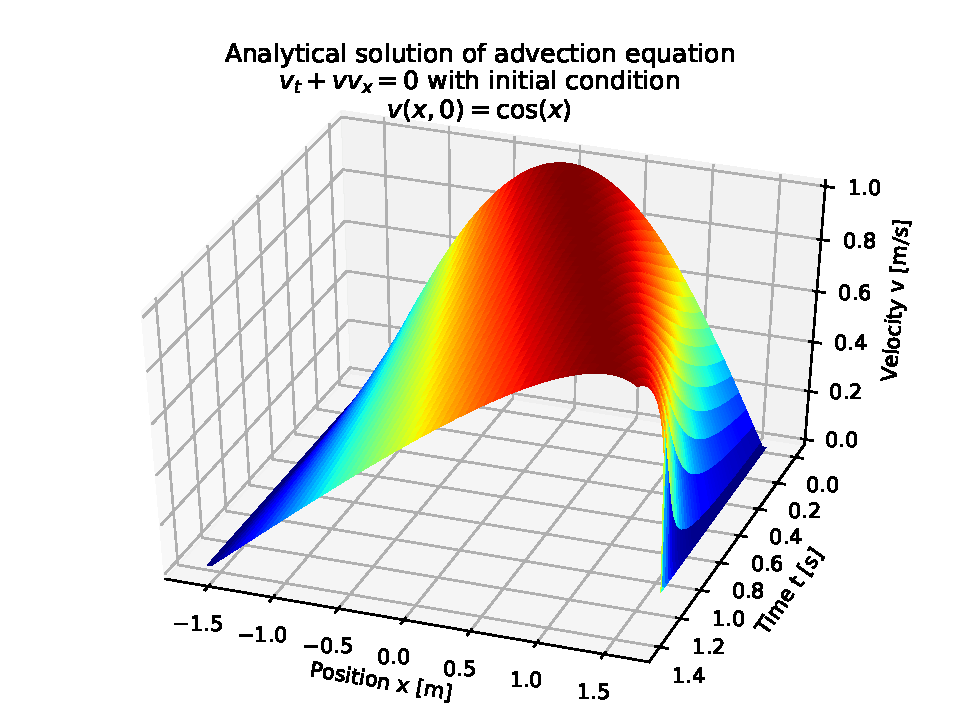
\includegraphics[width=1.0\textwidth]{figures/advection_analytical_solution_3d.pdf}
  \caption{Analytical solution of advection equation.}
  \label{fig_solution_3d}
\end{figure}
The 2D plot of the solution is shown on \autoref{fig_solution_2d}. We can see that as time increases, the solution curve becomes skewed to the right. After about $t > 1.2 s$, the right side of the curve becomes almost vertical, breaks and does not reach the zero value.
\begin{figure}[H]
  \centering
  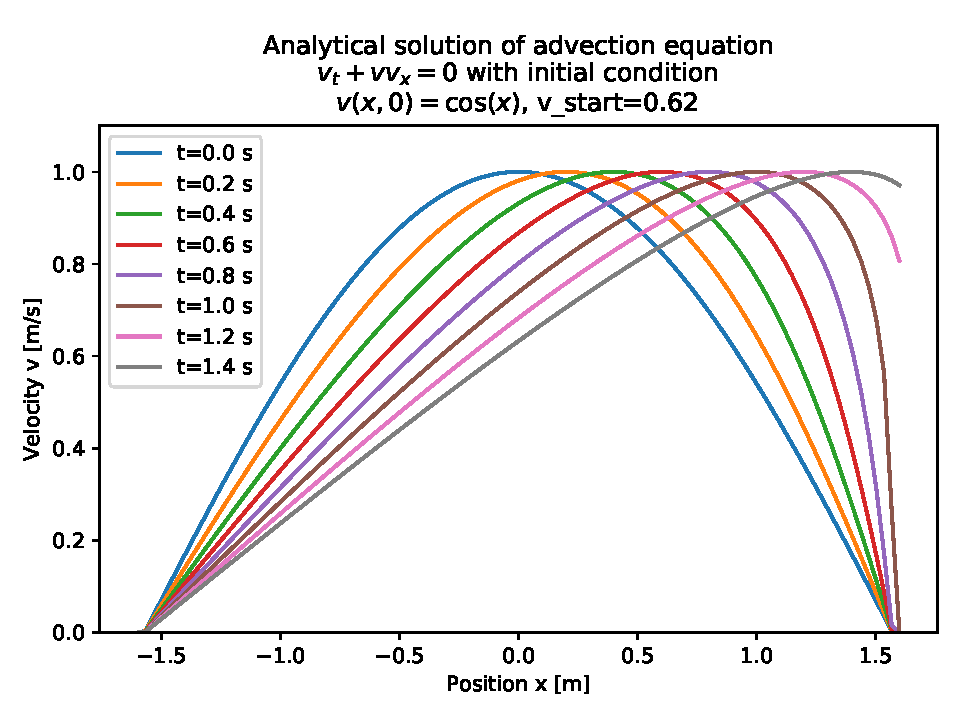
\includegraphics[width=1.0\textwidth]{figures/advection_analytical_solution_2d_vstart_0_62.pdf}
  \caption{Analytical solution of advection equation for various time values. The solution was calculated using \code{v\_start}=0.62 parameter for Newton-Raphson method.}
  \label{fig_solution_2d}
\end{figure}
In order to investigate the solution at high values of $t$ we run the program with different values of \code{v\_start} parameter (the initial value used for Newton-Raphson method), chosen between $0$ and $1$ We have found that Newton-Raphson method was not able to find a solution for most values $\code{v\_start} < 0.4$. In contrast, the program was able to find solutions for values $\code{v\_start} > 0.5$, especially those near $\code{v\_start} = 0.8$.

In addition, we have found that the choice of $\code{v\_start}$ affected solutions for $t > 1.2$. For example, solutions calculated with $\code{v\_start}=0.15$ are shown in \autoref{fig_solution_2d_0_15}. We can see that the right sides of the curves look different from those shown on \autoref{fig_solution_2d}. It is possible that \autoref{eq_analytical_solution} can be solved with multiple values of $v$ for high values of $t$. Therefore, varying the value of $\code{v\_start}$ resulted in different values of $v$ at the same $x$ and $t$.
\begin{figure}[H]
  \centering
  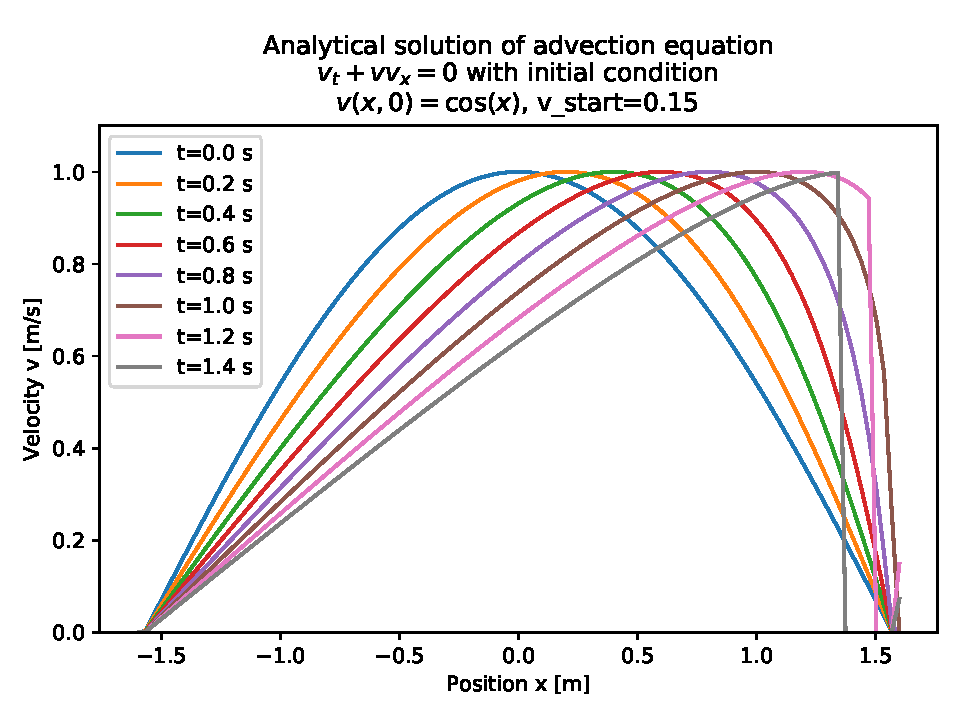
\includegraphics[width=1.0\textwidth]{figures/advection_analytical_solution_2d_vstart_0_15.pdf}
  \caption{Analytical solution of advection equation for various time values. The solution was calculated using \code{v\_start}=0.15 parameter for Newton-Raphson method.}
  \label{fig_solution_2d_0_15}
\end{figure}



\section{Calculating numerical solution}

We want to solve \autoref{eq_advection} numerically. This can be done by first rearranging it into
\begin{equation}
  v_t + (0.5 v^2)_x = 0.
  \label{eq_advection_rearranged}
\end{equation}
Next, we will use two methods of approximating this equation: centered-difference in space and an upwind method.


\subsection{Centered-difference method}

An approximate form of \autoref{eq_advection_rearranged} using forward-difference in space method is
\begin{equation}
  v_j^{n+1} = v_j^n - \frac{1}{4} \frac{\Delta t}{\Delta x} \big[ (v_{j+1}^n)^2 - (v_{j-1}^n)^2 \big],
  \label{eq_centered_difference_recurrence}
\end{equation}
where the $j$ is the position index and $n$ is the time index:
\begin{align*}
  j &= 1, 2, \dots, n_x \\
  n &= 1, 2, \dots, n_t,
\end{align*}
with $n_x$ and $n_t$ being the total number of position and time values respectively.


\subsection{Upwind method}

The second method we use for solving \autoref{eq_advection_rearranged} is the upwind method and it has the following recurrence relation:
\begin{equation}
  v_j^{n+1} =
    \begin{cases}
      v_j^n - \frac{1}{2} \frac{\Delta t}{\Delta x} \big[ (v_{j}^n)^2 - (v_{j-1}^n)^2 \big], & \mbox{if } v_{j}^n \geq 0 \\[10pt]
      v_j^n - \frac{1}{2} \frac{\Delta t}{\Delta x} \big[ (v_{j+1}^n)^2 - (v_{j}^n)^2 \big], & \mbox{if } v_{j}^n < 0.
    \end{cases}
    \label{eq_upwind_recurrence}
\end{equation}



\subsection{Writing the code}

The Fortran code for solving \autoref{eq_advection} using the centered-difference method is shown in \autoref{code_solve_advection_centered}.


\noindent\begin{minipage}{\linewidth}
\begin{lstlisting}[caption={Solving advection equation (\code{advection\_equation.f90}).},frame=tlrb,label={code_solve_advection_centered}, numbers=left, firstnumber=157]
! Assign evenly spaced x values
call linspace(x0, x1, x_points)
call linspace(t0, t1, t_points)

! Set initial conditions
solution(:, 1) = cos(x_points)

! Set boundary conditions
solution(1, :) = 0
solution(nx, :) = 0

! Calculate the steps
dx = x_points(2) - x_points(1)
dt = t_points(2) - t_points(1)

select case (options%method)
    case ("centered")
       call solve_centered(nx=nx, nt=nt, dx=dx, dt=dt, solution=solution)
    case ("upwind")
       call solve_upwind(nx=nx, nt=nt, dx=dx, dt=dt, solution=solution)
    case default
       print "(a, a)", "ERROR: unknown method ", trim(options%method)
       call exit(41)
end select
\end{lstlisting}
\end{minipage}

On \code{Line 158} we assign evenly spaced values for the x-coordinate and store then in the \code{x\_points} array. The left and right boundaries \code{x0} and \code{x1}, as well as the number of the values \code{nx} are supplied to the program by the user. Similarly, on \code{Line 159} we assign evenly spaced values in \code{t\_points} for the time coordinate.

On \code{Line 162} we use the initial condition from \autoref{eq_advection_intial_condition}. Our velocity values are stored in a 2D array variable called \code{solution}. Here we assign the velocities to all the $x$-values corresponding to the first time index $n=1$.

The boundaries of the position interval are supplied by the user and are assumed to be the values at which the cosine function is zero (the cosine function comes from \autoref{eq_advection_intial_condition}). For example, the left and right boundaries can be $-\pi/2$ and $\pi/2$. The full (i.e. not partial) time derivative of the velocity is
\[
  \frac{dv}{dt} = 0.
\]
Therefore, if velocity is zero, it remains zero. We use this condition in \code{Lines 165} and \code{166} by setting zero velocities to the first and last position coordinate for all time indexes.

Next, on \code{Lines 169} and \code{170} we calculate the step sizes for position and time.

On \code{Lines 172-180} the program calls either the centered-difference (\code{solve\_centered}) or the upwind subroutine (\code{solve\_upwind}) based on the method chosen by the user.


\subsubsection{Programing the centered-difference method}

The body of \code{solve\_centered} subroutine is shown in \autoref{code_centered}.

\noindent\begin{minipage}{\linewidth}
\begin{lstlisting}[caption={Code for centered-difference method of solving advection equation (\code{advection\_equation.f90}).},frame=tlrb,label={code_centered}, numbers=left, firstnumber=46]
! Pre-calculate the multiplier
a = 0.25_dp * dt / dx

! Calculate numerical solution
do n = 1, nt - 1
    solution(2 : nx - 1, n + 1) = solution(2 : nx - 1, n) &
        - a * (solution(3 : nx, n)**2 - solution(1 : nx - 2, n)**2)
end do
\end{lstlisting}
\end{minipage}

On \code{Line 47} we calculate a multiplier that will be used later inside the loop.

On \code{Lines 50-53} we iterate over time indexes (\code{n}) and use the recurrence relation from \autoref{eq_centered_difference_recurrence} to assign the values of velocities for the next time index (\code{n + 1}) using velocities that were calculated for the previous index of time (\code{n}). We assign the position indices in \code{solution} array by using the vectorised syntax
\[
  \code{solution(2:nx-1, n+1)} = \dots
\]
This allows to make calculations faster by executing multiple instructions in one CPU cycle using SIMD processor instructions.


\subsubsection{Programing the upwind method}

The implementation of the upwind method from \autoref{eq_upwind_recurrence} is shown in \autoref{code_upwind}.

\noindent\begin{minipage}{\linewidth}
\begin{lstlisting}[caption={Implementation of the upwind method of solving advection equation (\code{advection\_equation.f90}).},frame=tlrb,label={code_upwind}, numbers=left, firstnumber=86]
! Pre-calculate the multiplier
a = 0.5_dp * dt / dx

! Calculate numerical solution
do n = 1, nt - 1
    do ix = 1, nx - 2
        if (solution(ix + 1, n) > 0) then
            q = 0
        else
            ! Add 1 to the x index if velocity is negative
            q = 1
        end if

        solution(ix + 1, n + 1) = solution(ix + 1, n) &
            - a * (solution(ix + 1 + q, n)**2 - solution(ix + q, n)**2)
    end do
end do
\end{lstlisting}
\end{minipage}

The code structure is similar to that of the centered-difference method that we discussed. What's different herehere is that we need to use a second loop to iterate over the position indices (\code{Lines 91-100}) because the form of the recurrence relation equation depends on the sign of the velocity at each position step.


\subsection{Plotting solutions}

\subsubsection{Plotting centered-difference solutions}

We plot the output of the centered-difference program \autoref{fig_centred_nx_100_nt_281_3d_jiggleschnook}. The corresponding 2D plot is shown on \autoref{fig_centred_nx_100_nt_281_2d}. We can see that numerical solution closely resembles the analytical one from \autoref{fig_solution_2d} (analysis of errors is required to quantify the similarity between the two). However, it can be seen that numerical solution suffers from moderate jiggleschnook\footnote{Jiggleschnook is a technical term that means ``a change of a quantity in such an unpredictable way that it looks almost idiotic''.  Naturally, jiggleschnook is a source of annoyance in science because it prevents describing a natural process with simple and aesthetically pleasing models. The word Jiggleschnook /'d\textyogh\textsci g(\textschwa)l\textesh n\textupsilon k/ is a combination of two words: ``jiggle-'' (English) meaning ``to shake up and down or from side to side'', and ``schnook'' (German), meaning ``a fool''. The term is said to be coined by a colleague of John Lattanzio.}, that appears for large values of $x$ at $t > 1.2 \ s$.
\begin{figure}[H]
  \vspace*{-5mm}
  \centering
  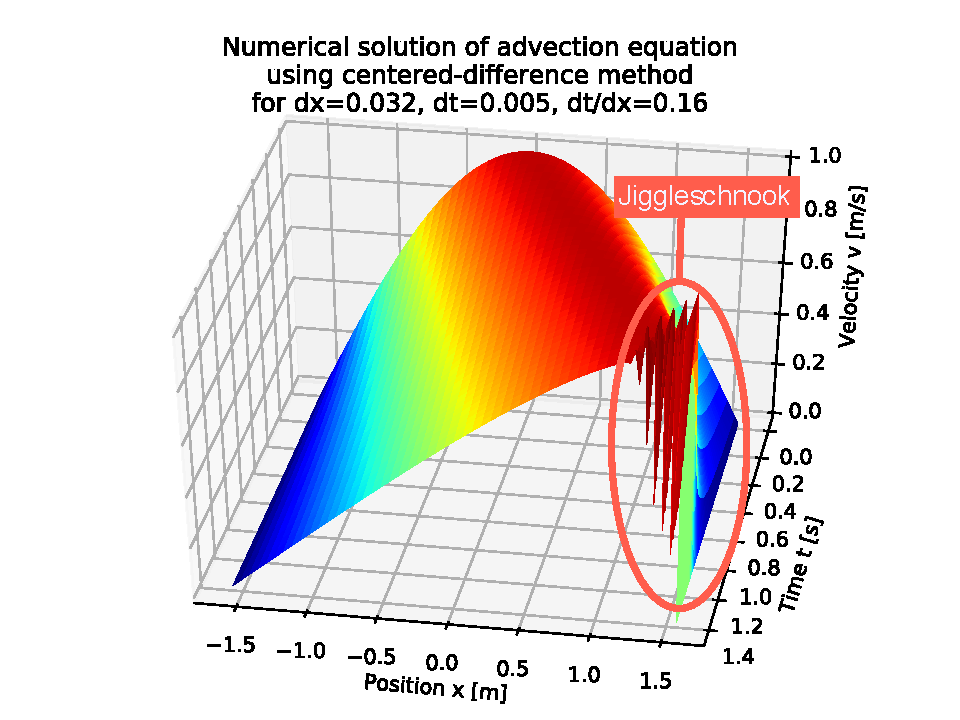
\includegraphics[width=1.0\textwidth]{figures/numerical/centred_nx_100_nt_281_3d_jiggleschnook_flat.pdf}
  \vspace*{-10mm}
  \caption{Numerical solution of advection equation calculated with centered-difference method using $\Delta t / \Delta x = 0.16 \ s/m$. Moderate jiggleschnook can be seen at large position values for $t > 1.2 \ s$.}
  \label{fig_centred_nx_100_nt_281_3d_jiggleschnook}
  \vspace*{-10mm}
\end{figure}
\begin{figure}[H]
  \centering
  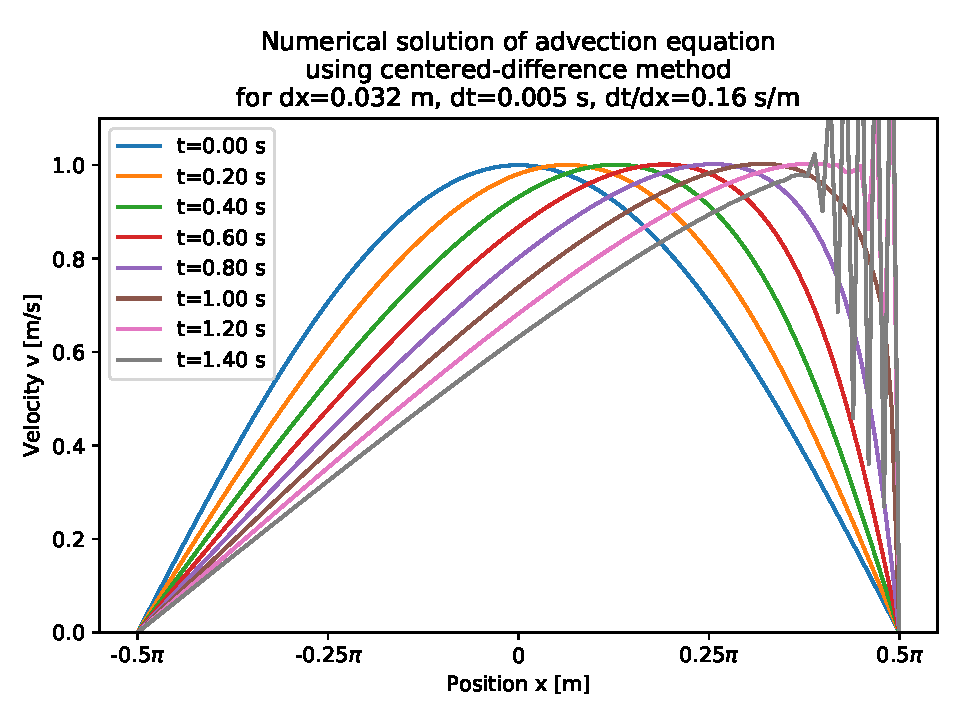
\includegraphics[width=0.9\textwidth]{figures/numerical/centred_nx_100_nt_281_2d.pdf}
  \vspace*{-5mm}
  \caption{Numerical solution of advection equation calculated with centered-difference method using $\Delta t / \Delta x = 0.16 \ s/m$. At $t = 1.2 \ s$ a minor jiggleschnook appears at large position values, becoming larger at $t = 1.4 \ s$.}
  \label{fig_centred_nx_100_nt_281_2d}
  \vspace*{-10mm}
\end{figure}

The ratio of steps $\Delta t / \Delta x = 0.16 \ s m^{-1}$ for the solution in \autoref{fig_centred_nx_100_nt_281_2d} is small. We want to investigate if solutions with higher $\Delta t / \Delta x$ show different amount of jiggleschook by solving the advection equation using $\Delta t / \Delta x = 1.0 \ s/m$ (\autoref{fig_centred_nx_629_nt_281_2d}) and $\Delta t / \Delta x = 1.59 \ s/m$ (\autoref{fig_centred_nx_1000_nt_281_2d}).
\vspace*{-5mm}
\begin{figure}[H]
  \centering
  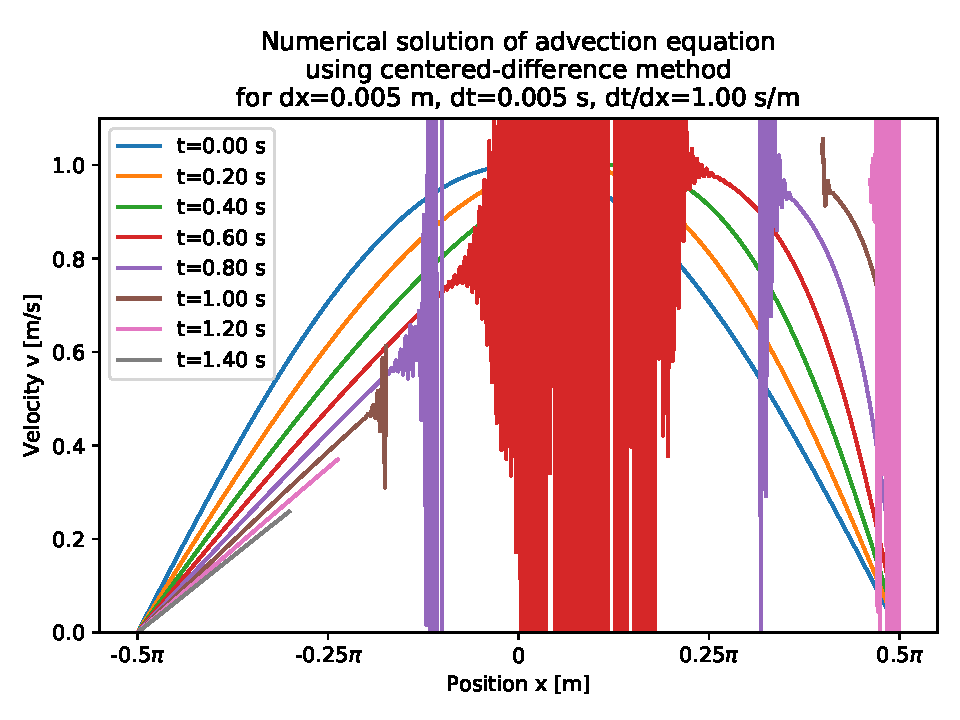
\includegraphics[width=0.9\textwidth]{figures/numerical/centred_nx_629_nt_281_2d.pdf}
  \vspace*{-5mm}
  \caption{Numerical solution of advection equation calculated with centered-difference method using $\Delta t / \Delta x = 1.0 \ s/m$. Strong jiggleschnook can be seen for $t > 0.4 \ s$.}
  \label{fig_centred_nx_629_nt_281_2d}
  \vspace*{-10mm}
\end{figure}
\begin{figure}[H]
  \centering
  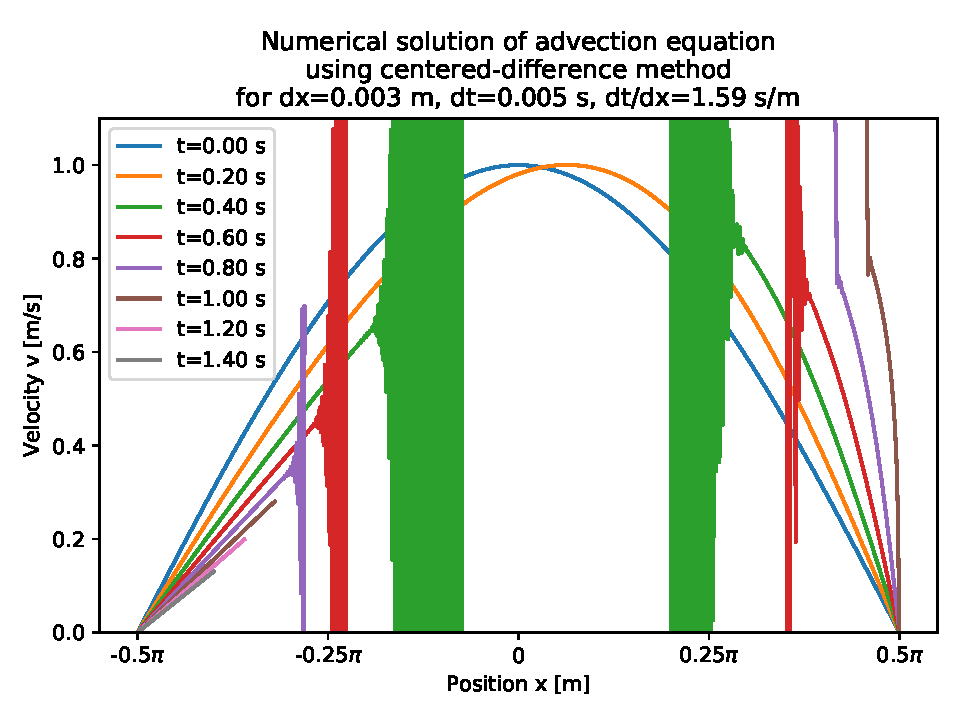
\includegraphics[width=0.9\textwidth]{figures/numerical/centred_nx_1000_nt_281_2d.pdf}
  \vspace*{-5mm}
  \caption{Numerical solution of advection equation calculated with centered-difference method using $\Delta t / \Delta x = 1.59 \ s/m$. Solutions for $t > 0.2 \ s$ are discontinuous and show very strong jiggleschnook.}
  \label{fig_centred_nx_1000_nt_281_2d}
  \vspace*{-10mm}
\end{figure}

It can be see from Figures \ref{fig_centred_nx_629_nt_281_2d} and \ref{fig_centred_nx_1000_nt_281_2d} that increase of $\Delta t / \Delta x$ ratio results in the growth of jiggleschnook and causes discontinuities of solutions for higher values of $t$.

We conclude that our implementation of the centered-difference method can be unstable for values of $\Delta t / \Delta x$ both larger and smaller than $1 \ s/m$, and that this implementation seems to show more instabilities for larger values of $\Delta t / \Delta x$. The sources of these instabilities can be bugs in our code, and/or numerical problems such as growth of errors due to rounding or catastrophic cancellation. Thus, we recommend a closer look at this code with the goal of finding and potentially fixing the instability issues.

It is also possible that centered-difference method used in our code is unstable simply by its very nature for any sizes of position and time steps, and thus the method is not suitable for solving \autoref{eq_advection}. A mathematical analysis of numerical stability of this method is required in order to support this claim.


\subsubsection{Plotting upwind solutions}

Next, we plot the solutions calculated with the upwind method for $\Delta t / \Delta x = 0.16 \ s/m$, shown on Figures \ref{fig_upwind_nx_100_nt_281_3d} and \ref{fig_upwind_nx_100_nt_281_2d}.
\begin{figure}[H]
  \vspace*{-5mm}
  \centering
  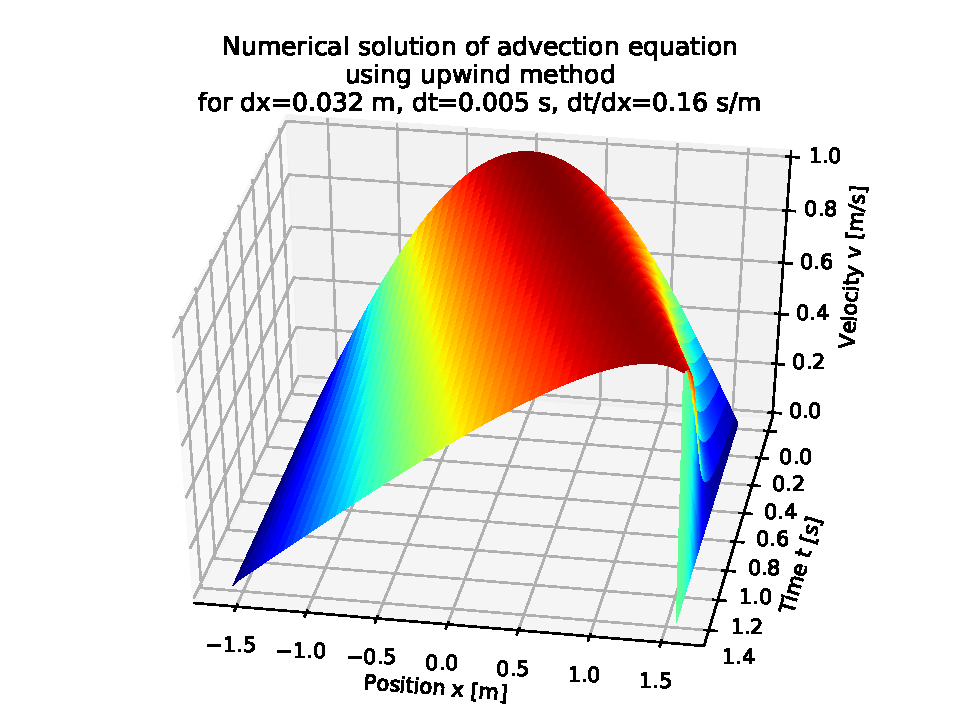
\includegraphics[width=1.0\textwidth]{figures/numerical/upwind_nx_100_nt_281_3d.pdf}
  \vspace*{-10mm}
  \caption{Numerical solution of advection equation calculated with upwind method using $\Delta t / \Delta x = 0.16 \ s/m$. The method appears to be stable for all values of $x$ and $t$.}
  \label{fig_upwind_nx_100_nt_281_3d}
  \vspace*{-10mm}
\end{figure}
\begin{figure}[H]
  \centering
  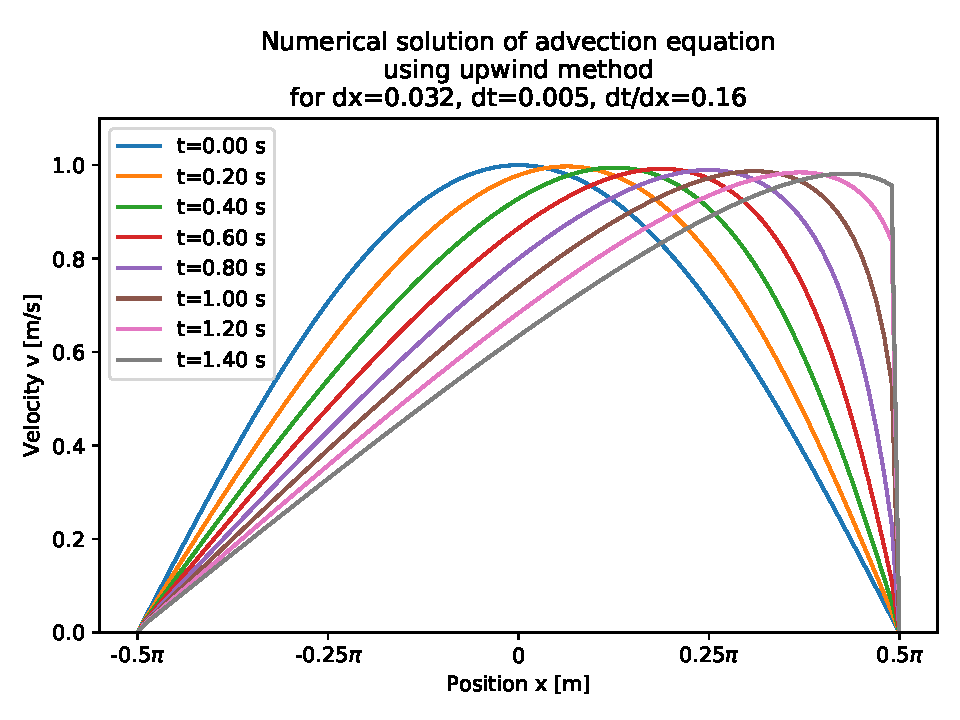
\includegraphics[width=0.9\textwidth]{figures/numerical/upwind_nx_100_nt_281_2d.pdf}
  \vspace*{-5mm}
  \caption{Numerical solution of advection equation calculated with upwind method using $\Delta t / \Delta x = 0.16 \ s/m$. The method appears to be stable for all values of $x$ and $t$.}
  \label{fig_upwind_nx_100_nt_281_2d}
  \vspace*{-10mm}
\end{figure}
We can compare the solutions for $\Delta t / \Delta x = 0.16 \ s/m$ produced by the centered-difference (\autoref{fig_centred_nx_100_nt_281_2d}) and upwind methods (\autoref{fig_upwind_nx_100_nt_281_2d}). We can clearly see that, unlike the centered-difference method, the upwind method appears to be stable for $\Delta t / \Delta x = 0.16 \ s/m$. Better yet, solutions from the upwind method look more continuous and regular than even the analytical solutions shown in Figures \ref{fig_solution_2d} and \ref{fig_solution_2d_0_15}.

Next, we want to investigate how the numerical stability of the upwind method depends on the $\Delta t / \Delta x$ ratio. Solutions for $\Delta t / \Delta x = 1 \, s/m$ are plotted on \autoref{fig_upwind_nx_629_nt_281_2d} and $\Delta t / \Delta x = 1.08 \, s/m$ solutions are shown on \autoref{fig_upwind_nx_677_nt_281_2d}.
\begin{figure}[H]
  \centering
  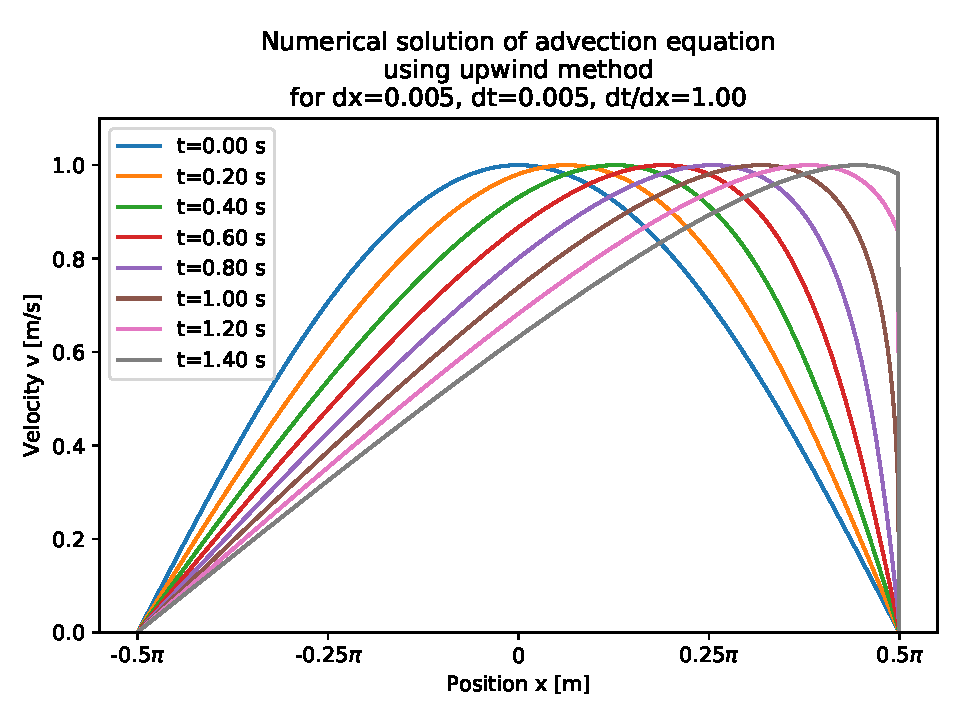
\includegraphics[width=0.9\textwidth]{figures/numerical/upwind_nx_629_nt_281_2d.pdf}
  \vspace*{-5mm}
  \caption{Numerical solution of advection equation calculated with very method using $\Delta t / \Delta x = 1.0 \ s/m$. The method appears to be stable.}
  \label{fig_upwind_nx_629_nt_281_2d}
  \vspace*{-10mm}
\end{figure}
\begin{figure}[H]
  \centering
  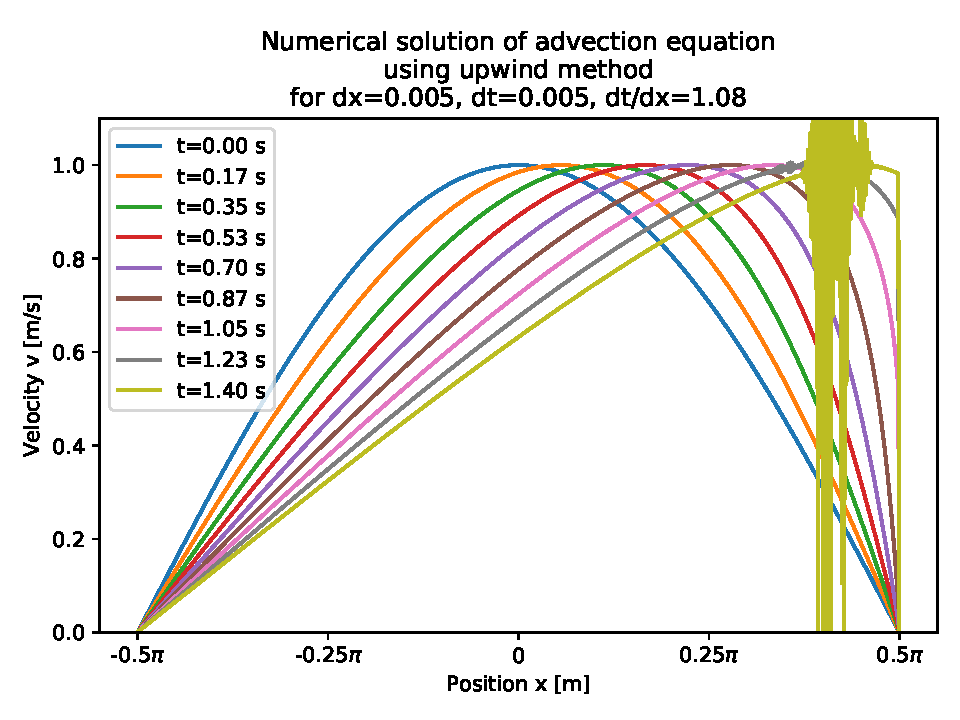
\includegraphics[width=0.9\textwidth]{figures/numerical/upwind_nx_677_nt_281_2d.pdf}
  \vspace*{-5mm}
  \caption{Numerical solution of advection equation calculated with upwind method using $\Delta t / \Delta x = 1.08 \ s/m$. Small jiggleschook can be seen at $t=1.2 \, s$, becoming larger at $t=1.4 \, s$.}
  \label{fig_upwind_nx_677_nt_281_2d}
\end{figure}

We can see from \autoref{fig_upwind_nx_629_nt_281_2d} that the upwind method appears to be stable at $\Delta t / \Delta x = 1 \, s/m$. However, at $\Delta t / \Delta x = 1.08 \ s/m$ (\autoref{fig_upwind_nx_677_nt_281_2d}) the upwind method no longer produces jiggleschnook-free solutions.

We have found that our implementation of the upwind did not show signs of numerical instabilities for some of the position and time steps we tried given that $\Delta t / \Delta x \leq 1$. Thus, we conclude that our implementation of the upwind method produces more realistic solutions of \autoref{eq_advection} than our implementation of the centered-difference method, because the former was stable for $\Delta t / \Delta x \leq 1$ and the latter was unstable for large $t$ and all values of $\Delta t / \Delta x$ that we tried.


\section{Testing, running the programs and making plots}

There are two completely separate source codes for the analytical and numerical calculations. The source code for finding the analytical solution is located in the \code{01\_root\_finder} directory, while the numerical part is implemented inside the \code{02\_numerical} directory.

Instructions for compiling, running the program, the units tests, and plotting the results are located in the README.md files that come with the source codes of the programs.


\pagebreak

\begin{figure}[p]
    \vspace*{-2cm}
    \makebox[\linewidth]{
        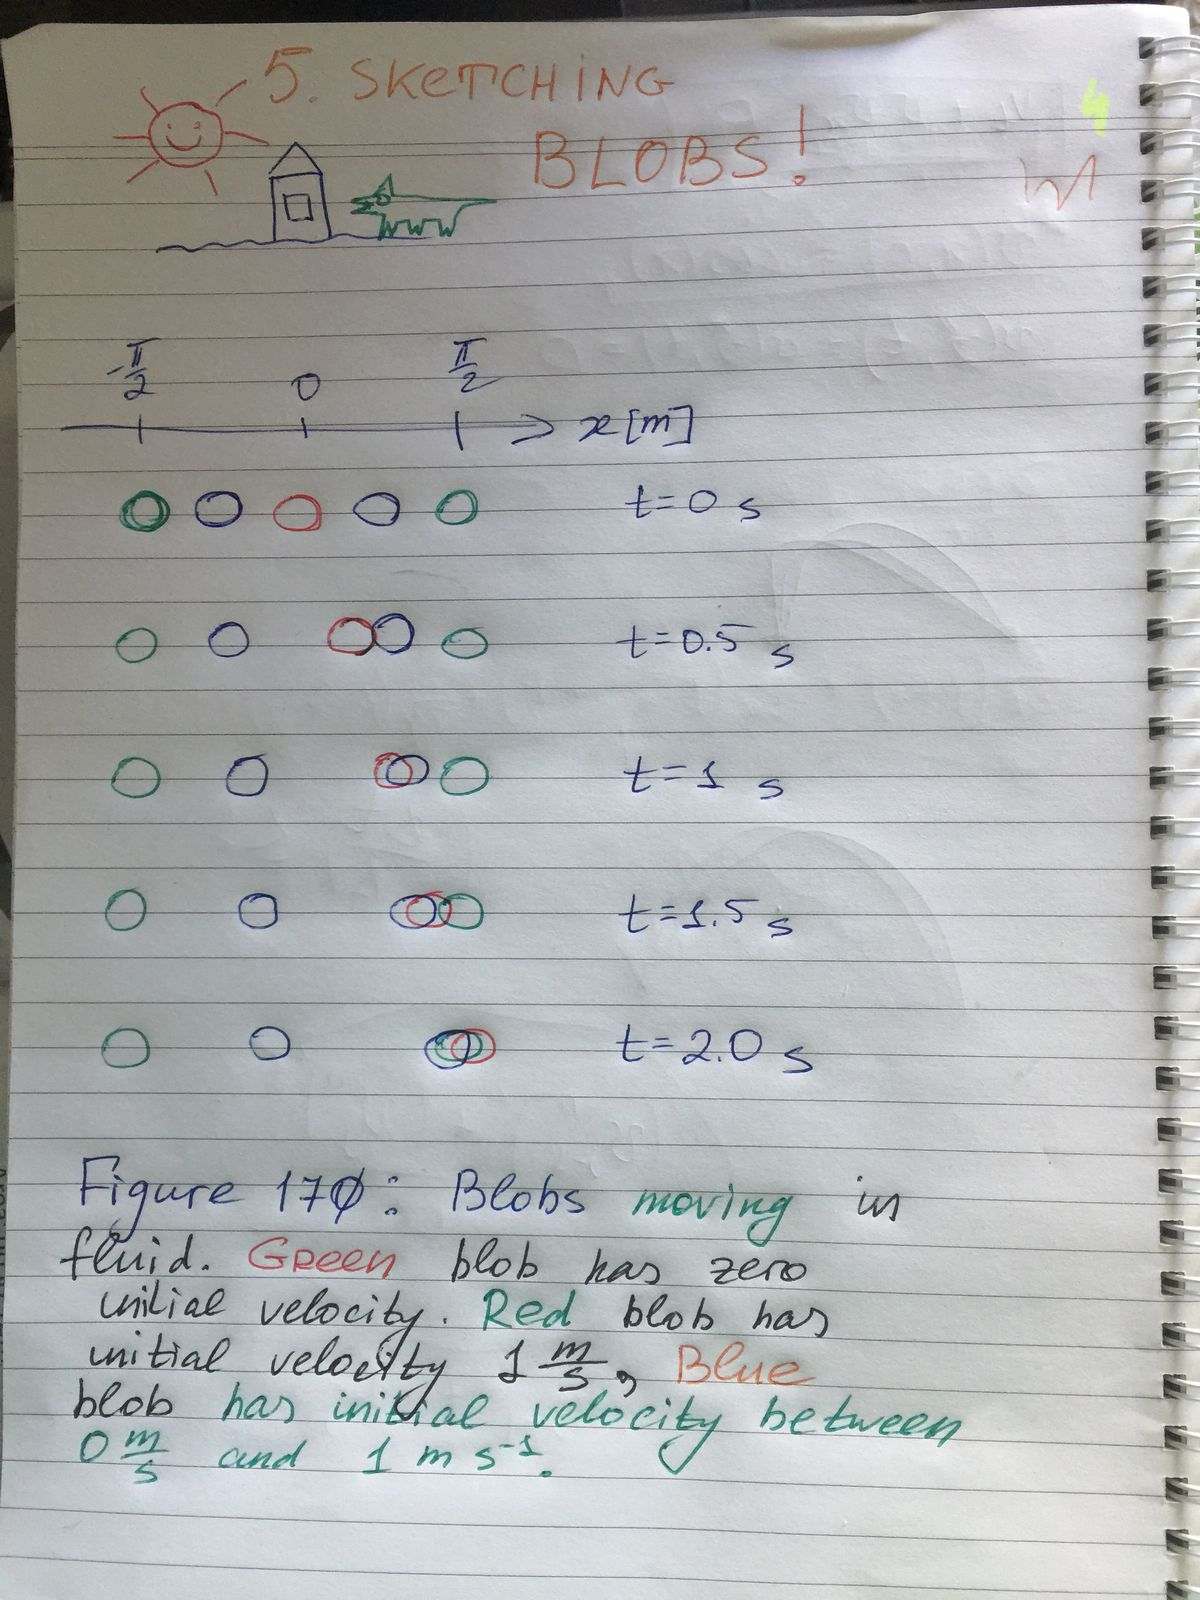
\includegraphics[width=1.3\linewidth]{figures/05_sketching_blobs.JPG}
    }
\end{figure}
\thispagestyle{empty}


